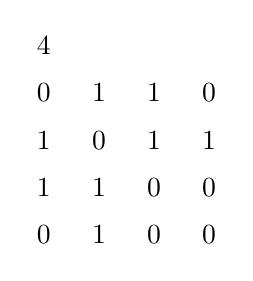
\begin{tikzpicture}[baseline=(current bounding box.center), x=0.7cm, y=0.6cm]
  % Entrada del programa: tamaño del grafo y matriz de adyacencia de G_{13}, como en el .txt
  \node at (1,0) {$4$};
  % Entradas: {fila/columna/valor}
  \foreach \fil/\col/\val in {1/1/0, 1/2/1, 1/3/1, 1/4/0,
                              2/1/1, 2/2/0, 2/3/1, 2/4/1,
                              3/1/1, 3/2/1, 3/3/0, 3/4/0,
                              4/1/0, 4/2/1, 4/3/0, 4/4/0}
    \node at (\col,-\fil) {$\val$};
\end{tikzpicture}
